\documentclass[11pt,b5paper,twoside,openany,final]{book}

\usepackage{ifpdf}

% [file: layout.tex, started: 18-March-2008]
%
% NOTES
%   This macro file contains page layout info for Ph.D. thesis
%
% CHANGES
%   2008.03.18	*	Started.

% ----- layout parameters ------------------------------------------------
\ifpdf
	\usepackage[dvips=false, pdftex=true, vtex=false]{geometry}
\else
	\usepackage[dvips=true, pdftex=false, vtex=false]{geometry}
\fi

% VU requirements 2021 m.
%puslapio dydis – B5 (17x24 cm),
%apatinė paraštė 2 cm, viršutinė paraštė 1,5 cm, kairė ir dešinė paraštės turi būti 2,5 cm,
%tarpai tarp eilučių – 1,15 intervalo,  (Rokas.: siuo metu paliktas defaultinis)
%pirmojo lygmens antraštė – 12 pt. Times New Roman; likusios paantraštės - 11 pt. Times New Roman,
%teksto šriftas – 11 pt. Times New Roman,
\geometry{%
 	b5paper,
    paperwidth=170mm, 
    paperheight=240mm,
 	bindingoffset=0pt,
 	centering,
 	hmargin=25mm,
    bottom=20mm,
    top=15mm%,
 	%includehead,
 	%includefoot
}  
  
\raggedbottom                           % height of text may vary per page

%\iffalse
\newlength{\oldparindent}
\newlength{\oldparskip}

\newcommand{\IZParagraph}{%
    \setlength{\oldparindent}{\parindent}
    \setlength{\oldparskip}{\parskip}
    \setlength{\parindent}{5mm}            % no indent
    \setlength{\parskip}{2ex plus 0.5ex minus 0.2ex}    % space between paragraphs
}

\newcommand{\restoreParagraph}{%
    \setlength{\parindent}{\oldparindent}
    \setlength{\parskip}{\oldparskip}
}
%\fi

%% VU requirements
%% 1.15 linespacing, bet paliktas defaultinis
%\linespread{1.15}
\usepackage{setspace}
%\onehalfspacing

	
\ifpdf
\usepackage[pdftex]{hyperref,graphicx} % pdf references support

\hypersetup{%
	pdfauthor   = {Rokas Astrauskas},
	pdftitle    = {COMPUTER MODELLING OF DIFFUSION - REACTION EQUATIONS},
	pdfsubject  = {PhD Thesis},
	pdfkeywords = {},
	pdfcreator  = {LaTeX with hyperref package},
	pdfproducer = {pdflatex},
	breaklinks  = {true},
	pdfstartview = {FitH},
	bookmarksnumbered = {true},
	bookmarksopen = {true},	
	bookmarksopenlevel = 2,
	plainpages={false},
	pdfpagetransition={Dissolve},	
	colorlinks = {true}, %defaultinis, padaro spalvotus staciakampius ant visu linku. Uzdejus true, bus tik spalvos ant skaiciu. Turbut graziau atrodo tik spalvos.
	%Norint nespalvotu nuorodu i formules, literatura, etc:
	%linkcolor = {black},
	%citecolor = {black},
	%filecolor = {black},
	%pilkos atspalviai:
	%linkcolor = [rgb]{0.3, 0.3, 0.3},
	%citecolor = [rgb]{0.6, 0.6, 0.6},
	%filecolor = [rgb]{0.3, 0.3, 0.3},
	%runcolor = [rgb]{0.3, 0.3, 0.3},
}
\else
\usepackage[dvips,ps2pdf]{hyperref,graphicx} % pdf references support
\fi

% ----- packages ---------------------------------------------------------
\renewcommand{\contentsname}{Table of Contents}
%\usepackage[british]{babel}		% british-english style
%------ ikeliau is preambule-santrauka
%\usepackage[L7x]{fontenc}
%\usepackage[utf8]{inputenc}
\usepackage[T1]{fontenc}
\usepackage{aeguill}
\usepackage[lithuanian, british]{babel}
\usepackage{ogonek}  %komandai \k kuri uzdeda kableli ant raidziu
\newcommand{\british}{\selectlanguage{british}}
\newcommand{\lithuanian}{\selectlanguage{lithuanian}}
%-----
%Sprendimas į raidei
\usepackage{newunicodechar}
%\newunicodechar{Į}{\k{I}}
%\newunicodechar{į}{\k{i}}

\usepackage{amssymb}					% extra AMS math symbols
\usepackage{amsfonts}					% extra AMS math symbols
\usepackage{amsmath}					% AMS 
\usepackage[mathscr]{euscript}

\usepackage{xcolor}				% colors support
\renewcommand{\topfraction}{0.85}	%% 85% of page can contain figure
\renewcommand{\textfraction}{0.1}	%% 10% of page can contain text
\renewcommand{\floatpagefraction}{0.75}	%% 75% of page should be figure to be only float page

\usepackage[square,comma,numbers,sort&compress]{natbib}	% citations
\setlength{\bibsep}{0ex}

\usepackage{fancyhdr}		% fancy headings and footers

\usepackage{sectsty}			% change sections fonts									
\setcounter{secnumdepth}{3}	% depth of enumerated sections

\ifpdf
	\usepackage{microtype}		% experimental
\else
\fi

\usepackage{makeidx}			% index package
\makeindex								% generate index entries
%\usepackage{fix2col}			% fix two-column marks
\makeatletter
\renewenvironment{theindex}
	{%
	\if@twocolumn
  	\@restonecolfalse
  \else
  	\@restonecoltrue
	\fi
	%
	\columnseprule \z@
	\columnsep 25\p@
	\twocolumn[\@makeschapterhead{\indexname}]%
	\@mkboth{\MakeUppercase\indexname}%
					{\MakeUppercase\indexname}%
	\thispagestyle{plain}\parindent\z@
	\parskip\z@ \@plus .3\p@\relax			
	\let\item\@idxitem	
	}
	{\if@restonecol\onecolumn\else\clearpage\fi}
%%

\renewcommand\@idxitem{\par\hangindent 30\p@}
\renewcommand\subitem{\@idxitem \hspace*{10\p@}}
\renewcommand\subsubitem{\@idxitem \hspace*{20\p@}} 

\renewcommand{\see}[2]{\emph{\seename}~{#1}}
\newcommand{\justsee}[2]{{#1}}


\makeatother	% macros for dictionary like index			

\usepackage{palatino}				% IZ selection
\usepackage[T1]{fontenc}		% modern tex fonts

\usepackage{verbatim} %IZ: multiline komentams 

\usepackage{paralist}
\usepackage{tabularx}
\usepackage{booktabs}
\usepackage{multirow}
\setlength{\belowcaptionskip}{5pt}

\usepackage{rotating}	

\usepackage{epigraph}	

\usepackage{hyphenat}

\usepackage{pdfpages}   %Prikabina isorinius pdfus prie latex pdfo

\usepackage{array}
\usepackage{float}

\usepackage{siunitx}   %paketas skaiciams ir SI vienetams vaizduoti. Galima ir nenaudoti, bet aukstesnis lygis
\usepackage{textcomp}  %senas paketas, bet reikalingas kad nemestu kai kuriu siunitx klaidu
\sisetup{load-configurations = abbreviations}
\setlength{\headheight}{19pt}  %kazkokia problema su headheight

%Reikia sablonui. Galima istrinti
\usepackage[version=4]{mhchem}
\DeclareSIUnit \uM{\micro M}
\DeclareSIUnit \mM{\milli M}




% ----- macros ---------------------------------------------------------
\def\interpti{\relax}%
\def\invardinti#1{%
     \trivlist\item[\hskip\labelsep{\bfseries#1}}%]
\def\atstumti{\endtrivlist}%\interpti}
\newif\ifRoman
\def\Fshape{\ifRoman\rmfamily\else\itshape\fi}
\newcommand{\trivardis}[3]{\invardinti{#1\ #2}\ (#3).]\Fshape}
\newcommand{\dvivardis}[2]{\invardinti{#1\ #2.}]\Fshape}
\makeatletter
\let\@opargbegintheorem\trivardis
\let\@begintheorem\dvivardis
\let\@endtheorem\atstumti
\newcommand{\newproclaim}[3]{\newenvironment{#1}{\global\finishedfalse
   \Romantrue\@thm{#2}{#3}}{\finish\atstumti}}
\makeatother
\newif\iffinished\finishedtrue
\newcommand{\finish}{\iffinished\else\ifhmode\nolinebreak\fi\nopagebreak%
   \qquad\ifhmode\nolinebreak\fi\nopagebreak%
   \ensuremath{\square}\global\finishedtrue\fi}

\newtheorem{claim}{Proposition}[section]
\newtheorem{corollary}[claim]{Corollary}
\newtheorem{theorem}[claim]{Theorem}
\newtheorem{lemma}[claim]{Lemma}
\newproclaim{definition}{claim}{Definition}
\newproclaim{example}{claim}{Example}
\newproclaim{remark}{claim}{Remark}
\newproclaim{notation}{claim}{Notation}
\newenvironment{proof}{\invardinti{Proof.}\global\finishedfalse]}{\finish\atstumti}
\newenvironment{princ}[1]{\invardinti{#1}]\itshape}{\atstumti}
\newenvironment{prule}[1]{\paragraph{#1}\equation}
                         {\endequation\addvspace{1ex plus.2ex minus .2ex}}


\newcommand{\allmoodsA}{\ensuremath{:\mkern-4mu-\allmoodslipsA}}
\newcommand{\allmoodsB}{\ensuremath{:\mkern-4mu-\mkern-3mu\allmoodslipsB}}
\newcommand{\allmoodslipsA}{\ensuremath{)\mkern-7.3mu|\mkern-7mu(}}
\newcommand{\allmoodslipsB}{\ensuremath{)\mkern-4.8mu|\mkern-4.4mu(}}

\newenvironment{Abstract}{%
	\begin{center}
		\textbf{Abstract}%
 	\end{center}
 	\small \it \begin{quote}
}
{\end{quote}}
\newcommand{\IZheading}[1]{\scriptsize{\textit{#1}}}

\pagestyle{fancy}
\renewcommand{\chaptermark}[1]{\markboth{\thechapter.\ #1}{}}
\renewcommand{\sectionmark}[1]{\markright{\thesection.\ #1}}
%\renewcommand\thechapter{\arabic{section}}
%\renewcommand\thesection{\arabic{section}}

% \def\thechapter{\arabic{chapter}}

% \newcommand{\IZThesisHeadings}{%
% 	\fancyhead{}\fancyhead[LE]{\IZheading{\IZheading{\leftmark}}}\fancyhead[RO]{\IZheading{\rightmark}}
% 	\fancyfoot{}
% 	\fancyfoot[c]{\thepage}
% 	\fancypagestyle{plain}{%
% 		\fancyhf{}
% 		\fancyfoot[c]{\thepage}
% 		\renewcommand{\headrulewidth}{0pt}
% 	}
% }

\makeatletter
\def\cleardoublepage{%
	\clearpage\if@twoside \ifodd\c@page\else%
	\hbox{}%
	\thispagestyle{empty}%
	\newpage%
	\if@twocolumn\hbox{}\newpage\fi\fi\fi
}

\makeatother
    
\makeatletter	
\newcommand{\itemhdr}[1]{\par\hangindent 30\p@\relax{#1}\markboth{#1}{#1}}
\makeatother

\newcommand{\indexmarks}{%
	\fancyhead[R]{\IZheading{\leftmark}}
	\fancyhead[L]{\IZheading{\rightmark}}
}

\newcommand{\parammarks}[1]{%
	\fancyhead{}
	\fancyhead[RO,LE]{}
	\fancyhead[RO,LE]{\IZheading{#1}}
	\fancyfoot{}
	\fancyfoot[c]{\thepage}
	\fancypagestyle{plain}{%
		\fancyhf{}	
		\fancyfoot[c]{\thepage}
	\renewcommand{\headrulewidth}{0pt}
	}
}


%Rename default Contents table name
\addto\captionsbritish{\renewcommand{\contentsname}{Table of Contents}}

\begin{document}

%\frontmatter %command makes the pages numbered in lowercase roman

%%%%%%%%%%%%%%%%%%%%%%%%%%%%%%%%%%%%%%%%%%%%%%%%%%%%%%%%%%%%%%%%%%%%%%%%%%%%%%%%%%%%%%%%
%% Tile page in English or Lithuanian.
%% The First title is in English and the second one in Lithuanian
%% Please copy place the pages places if you change to first title Lithuanian and second English
%% All variables used in this file are defined in settings.text file / Visi kintamieji yra nurodyti settings.tex faile

%% Set page style, font family and line spacing 
\thispagestyle{empty}                   % no headers and footers
{\fontfamily{ptm}\selectfont
\linespread{1.15}\selectfont
% Nustatome šrifto dydį, plotį, žr. https://tex.stackexchange.com/questions/68745/possible-values-for-fontseries-and-fontshape
\renewcommand\bfdefault{m}% \renewcommand\bfdefault{bc} does not work and changes to m (Medium (normal))

%%%%%%%%%%%%%%%%%%%%%%%%%%%%%%%%%%%%%%%%%%%%%%%%%%%%%%%%%%%%%%%%%%%%%%%%%%%%%%%%%%%%%%%%
%% Tile page in English

\begin{flushright}
    \thesisDOI \\
    \thesisORCID
\end{flushright}

\begin{center}
	\vspace*{5mm}	
	\begin{flushleft}
         \fontsize{12}{12}\selectfont
	       VILNIUS UNIVERSITY \\
	\end{flushleft}
 
	\vspace{50mm minus 45mm}
	\begin{flushleft}
	   {\fontsize{15}{15}\selectfont  \thesisAuthorName  \  \thesisAuthorSurname \par}
    \end{flushleft}

	\vspace{10mm}
	\begin{flushleft}
    	{ \fontsize{21}{21}\selectfont
    	   \thesisTitleEN \par
    	}
    \end{flushleft}

    \vspace{70mm minus 45mm}
    \begin{flushleft}
        \renewcommand\bfdefault{b}
        \fontsize{12}{12}\selectfont
        {\bf DOCTORAL DISSERTATION}\\ 
    \end{flushleft}
    
    \vspace{5mm}
    \begin{flushleft}
%        \renewcommand\bfdefault{m}
        \fontsize{12}{12}\selectfont
%        \bf
            Natural Sciences, \\ %Mosklo sritis
            Informatics (N 009)  %Mokslo kryptis krypties kodas (kodas skliausteliuose, pvz., (N 001))
    \end{flushleft}
    
    \vspace{6mm}
    \begin{flushleft} 
         \fontsize{9}{9}\selectfont
        \bf VILNIUS \thesisYear
    \end{flushleft} 
\end{center}
}

\newpage
\thispagestyle{empty}                   % no headers and footers

%The dissertation was prepared between 20__ and 20__ (the name of the institution at which the dissertation was completed). The research was supported by (e.g. Research Council of Lithuania, if the doctoral studies were financed from the EU structural funds, or a scholarship was granted for academic accomplishments). 
%\begin{singlespace}
\noindent\nohyphens{The dissertation was prepared between {\thesisPreparationStartYear} and {\thesisYear} at Vilnius University.}
% (In case the doctoral dissertation is defended on an external basis, include the statement ‘The dissertation is defended on an external basis’).
% \vspace{0.5cm}
% \noindent{The dissertation is defended on an external basis.}

\vspace{1cm}
%The research was partially supported by the Research Council of Lithuania (Researcher groups projects Grant), project ... 
%Šita dalis, jeigu buvo papildomas finansavimas

% (If the dissertation is defended on an external basis, write ‘Academic consultant’) Prof. Habil. Dr. Name Surname (Name of institution, Research area, Research field, Field code). (In case the doctoral student had two academic supervisors, indicate the time frame(s) of their supervision).
\noindent {\bf Academic supervisor -- }{ \nohyphens{Prof. Habil. Dr. ...Name Surname..} (Vilnius University, Natural Sciences, Informatics -- N 009)}.\\
\noindent {\bf Academic consultant -- }{ \nohyphens{Prof. Dr. ...Name Surname..} (Vilnius University, Natural Sciences, Informatics -- N 009)}.\\ %(Name of institution, Research area, Research field, Field code).

\vspace{1cm}
\noindent
This doctoral dissertation will be defended in a public meeting of the Dissertation Defence Panel:

\vspace{0.5cm}
\noindent
{\bf Chairman  --} \nohyphens{{Prof. Dr. ...Name Surname...} (Vilnius University, Natural Sciences, Informatics -- N 009)}.\\ %(Name of institution, Research area, Research field, Field code).
{\bf Members:}\\ %[members are listed alphabetically by last name].
\nohyphens{Prof. ...Name Surname...}
(..., Natural Sciences, Informatics -- N 009).\\%(Name of institution, Research area, Research field, Field code)
\nohyphens{Prof. Dr. ...Name Surname...}
(..., Natural Sciences, Informatics -- N 009).\\
\nohyphens{Prof. Habil. Dr. ...Name Surname...} 
(..., Natural Sciences, Informatics -- N 009).\\
\nohyphens{Dr. ...Name Surname...}
(Tallinn University of Technology, Estonia, Natural Sciences, Chemistry -- N 003).\\

\vspace{2cm}
\noindent 
The dissertation shall be defended at a public meeting of the Dissertation Defense Panel at ..... a.m. on ...th .......... 20.. in room 203 of the Institute of Data Science and Digital Technologies of Vilnius University. \\
Address: Akademijos st. 4, LT-04812, Vilnius, Lithuania \\
Tel. +370 5 210 9300; e-mail: info@mii.vu.lt

\vspace{1cm}
\noindent
The text of this dissertation can be accessed at the Library of Vilnius
University, as well on the website of Vilnius University: \\ 
\href{https://www.vu.lt/lt/naujienos/ivykiu-kalendorius}{ \textit{\underline{https://www.vu.lt/lt/naujienos/ivykiu-kalendorius}}}.

%%%%%%%%%%%%%%%%%%%%%%%%%%%%%%%%%%%%%%%%%%%%%%%%%%%%%%%%%%%%%%%%%%%%%%%%%%%%%%%%%%%%%%%%
%% Title in Lithuanian language

\newpage
\thispagestyle{empty}                   % no headers and footers
{\fontfamily{ptm}\selectfont
\linespread{1.15}\selectfont
\renewcommand\bfdefault{m}
% Visi kintamieji yra nurodyti settings.tex faile / All constants are in settings.tex file
\begin{flushright}
    \thesisDOI \\
    \thesisORCID
\end{flushright}

\begin{center}
	\vspace*{5mm}	
	\begin{flushleft}
         \fontsize{12}{12}\selectfont
	       VILNIUS UNIVERSITETAS \\
	\end{flushleft}
 
	\vspace{50mm}
	\begin{flushleft}
	   {\fontsize{15}{15}\selectfont  \thesisAuthorName \  \thesisAuthorSurname \par}
    \end{flushleft}

	\vspace{10mm}
	\begin{flushleft}
    	{ \fontsize{21}{21}\selectfont
    	   \thesisTitleLT \par
    	}
    \end{flushleft}

    \vspace{50mm minus 45mm}
    \begin{flushleft}
        \renewcommand\bfdefault{b}
        \fontsize{12}{12}\selectfont
        {\bf DAKTARO DISERTACIJA}\\ 
    \end{flushleft}
    
    \vspace{5mm}
    \begin{flushleft}
        \renewcommand\bfdefault{m}
        \fontsize{12}{12}\selectfont
        \bf
            Gamtos mokslai, \\ %Mosklo sritis
            Informatika (N 009)  %Mokslo kryptis krypties kodas (kodas skliausteliuose, pvz., (N 001))
    \end{flushleft}
    
    \vspace{6mm}
    \begin{flushleft} 
         \fontsize{9}{9}\selectfont
        \bf VILNIUS \thesisYear
    \end{flushleft} 
\end{center}
}

\newpage
\thispagestyle{empty}                   % no headers and footers

% \begin{singlespace}
\noindent\nohyphens{Disertacija rengta {\thesisPreparationStartYear}--{\thesisYear} metais Vilniaus universitete.}

% Jei daktaro disertaciją gina eksternas įrašoma 
% \vspace{0.5cm}
% \noindent{Disertacija ginama eksternu.}
%Mokslinius tyrimus rėmė ...(pvz., Lietuvos mokslo taryba, jei doktorantūra buvo finansuojama ES struktūrinių fondų lėšomis ar buvo gauta stipendija už akademinius pasiekimus).

\vspace{1cm}
%Prie mokslinio vadovo ir konsultanto nurodoma: institucijos pavadinimas, mokslų sritis, mokslo kryptis, mokslo krypties kodas; jeigu buvo du doktoranto moksliniai vadovai, nurodomas vadovavimo laikotarpis).
\noindent {\bf Mokslinis (-ė) vadovas (-ė) --}{ {prof. dr. ...Vardas Pavardė... } (Vilniaus universitetas, gamtos mokslai, informatika -- N 009)}.

\noindent {\bf Mokslinis (-ė) konsultantas (-ė) -- }{ {prof. dr. ...Vardas Pavardė... } (Vilniaus universitetas, gamtos mokslai, informatika -- N 009)}.

\vspace{1cm}
\noindent
Gynimo taryba:  \\
{\bf Pirmininkas (-ė)} {-- {prof. dr. ...Vardas Pavardė...} (Vilniaus universitetas, gamtos mokslai, informatika -- N 009).\\}
{\bf Nariai:}\\ %[nariai surašomi abėcėlės tvarka pagal pavardes].
{prof. ...Vardas Pavardė...}
(..., gamtos mokslai, informatika -- N 009).\\
{prof. dr. ...Vardas Pavardė...}
(..., gamtos mokslai, informatika – N 009).\\
{prof. habil. dr. ...Vardas Pavardė...}
(..., gamtos mokslai, informatika - N 009).\\
{dr. ...Vardas Pavardė...}
(Talino technikos universitetas, Estija, gamtos mokslai, chemija -- N 003).


\vspace{2cm}
\noindent
%Disertacija ginama viešame / uždarame Gynimo tarybos posėdyje 20_ m. _____________ mėn. __ d. ____ val. (institucijos pavadinimas) fakulteto / instituto _______ posėdžių salėje / auditorijoje. Adresas: (gatvė, namo numeris, patalpos numeris, miestas, Lietuva), tel. +370__________ ; el. paštas 
Disertacija ginama viešame Gynimo tarybos posėdyje 20.. m. .......... ... d. ... val. Vilniaus universiteto Duomenų mokslo ir skaitmeninių technologijų instituto  203 auditorijoje. Adresas: Akademijos g. 4, LT\nobreakdash-04812, Vilnius, Lietuva, tel. +370 5 210 9300; el. paštas: info@mii.vu.lt.\\

\vspace{1cm}
\noindent
Disertaciją galima peržiūrėti Vilniaus universiteto bibliotekoje ir Vilniaus universiteto interneto svetainėje adresu: 
\href{https://www.vu.lt/lt/naujienos/ivykiu-kalendorius}{ \textit{\underline{https://www.vu.lt/lt/naujienos/} \underline{ivykiu-kalendorius}}}. 



\cleardoublepage
\restoreParagraph

\pagestyle{plain}

%%%%%%%%%%%%%%%%%%%%%%%%%%%%%%%%%%%%%%%%%%%%%%%%%%%%%%%%%%%%%%%%%%%%%%%%%%%%%%%%%%%%%%%%%%%%%%
%% This file includes Table of Contents

\phantomsection %The \phantomsection command is needed to create a link to a place in the document that is not a figure, equation, table, section, subsection, chapter, etc.

\tableofcontents % Table of Contents

%-------------- Prasideda pagrindine disertacijos dalis  ------------------
%-------------- Start of main thesis part  ------------------
\phantomsection
%\addcontentsline{toc}{chapter}{\numberline{}Notation}
%\parammarks{Notation}
\addcontentsline{toc}{chapter}{\MakeUppercase{Notation}}
\chapter*{Notation}

\begin{compactitem}[]
	\item $A$ amplitude caused by the feeding screw
	\item $a$ acceleration of a mass change
	\item $\alpha_1$ the weight of distance in space
	\item $\alpha_2$ the weight of distance in time
\end{compactitem}   %Pazymejimai/Notations

%\mainmatter %ommand changes the behavior back to the expected version, and resets the page number. 

\pagestyle{plain}
\IZParagraph

% NOTES to the author
% For chapter naming, please use APA style https://titlecapitalize.com/title-case-styles/
    % APA, or American Psychological Style, is one of the most commonly used title case styles in academia. It’s mainly used for research papers in social and behavioral sciences. 
    
    % Its title case rules are also easy enough to remember and follow. Capitalize all major words (nouns, pronouns, verbs, adjectives) in your title, as well as prepositions and conjunction with four or more letters. If your title includes a hyphenated word, capitalize both the initial letters before and after the hyphen. Lastly, the first word after a colon or dash is also capitalized when you’re following the APA style of capitalization for your title or headings.

\chapter*{Introduction / Įvadas}
\label{cha:intro}
\addcontentsline{toc}{chapter}{\MakeUppercase{Introduction / Įvadas}} 

Lorem ipsum dolor sit amet, consectetur adipiscing elit. Duis semper hendrerit faucibus. Donec mauris quam, condimentum quis velit et, sodales luctus arcu. Etiam eget rhoncus nunc, in tempus urna. Etiam dignissim quam libero, et aliquam urna tincidunt ac. Aliquam erat volutpat. Aliquam non urna nulla. Aliquam sodales porta tristique. Suspendisse efficitur ante non elit consectetur, et tincidunt nisl ultrices. Proin mollis eleifend lacus, ut fermentum justo porta a.

\phantomsection % Removes warning form hyperref package
\section*{Research area / Tyrimų sritis}
\addcontentsline{toc}{section}{Research Area / Tyrimų sritis} 

Lorem ipsum dolor sit amet, consectetur adipiscing elit. Duis semper hendrerit faucibus. Donec mauris quam, condimentum quis velit et, sodales luctus arcu. Etiam eget rhoncus nunc, in tempus urna. Etiam dignissim quam libero, et aliquam urna tincidunt ac. Aliquam erat volutpat. Aliquam non urna nulla. Aliquam sodales porta tristique. Suspendisse efficitur ante non elit consectetur, et tincidunt nisl ultrices. Proin mollis eleifend lacus, ut fermentum justo porta a.

Fusce convallis, ipsum sed suscipit tincidunt, lectus erat rhoncus lacus, quis faucibus dolor felis auctor felis. Suspendisse iaculis mi nec bibendum lobortis. Sed placerat eget tellus ut rutrum. Mauris finibus leo arcu, ut consectetur nisl condimentum eget. Donec bibendum eros orci, vel aliquam magna efficitur ac. Nulla sit amet luctus lorem, at viverra risus. Suspendisse scelerisque in arcu at ultrices. Aliquam nunc magna, aliquet quis 
accumsan quis, interdum id libero.

Praesent nisi neque, aliquam eu tempus vitae, faucibus nec est. Nam eu est vel risus aliquam luctus. Maecenas a urna at risus pharetra rutrum. Class aptent taciti sociosqu ad litora torquent per conubia nostra, per inceptos himenaeos. Aenean mauris nulla, commodo vitae dignissim nec, sagittis at tellus. Suspendisse potenti. Nullam a felis hendrerit, iaculis nisi volutpat, vehicula lacus. Ut ac sapien risus. Fusce commodo odio et fringilla egestas. Mauris at sollicitudin neque. In non maximus dui, ut rhoncus dolor. Etiam bibendum porta sem.


\section*{Actuality / Problemos aktualumas}
\addcontentsline{toc}{section}{Actuality / Problemos aktualumas} 

Lorem ipsum dolor sit amet, consectetur adipiscing elit. Duis semper hendrerit faucibus. Donec mauris quam, condimentum quis velit et, sodales luctus arcu. Etiam eget rhoncus nunc, in tempus urna. Etiam dignissim quam libero, et aliquam urna tincidunt ac. Aliquam erat volutpat. Aliquam non urna nulla. Aliquam sodales porta tristique. Suspendisse efficitur ante non elit consectetur, et tincidunt nisl ultrices. Proin mollis eleifend lacus, ut fermentum justo porta a.


\section*{Research Object / Tyrimo objektas}
\addcontentsline{toc}{section}{Research Object / Tyrimo objektas} 

Lorem ipsum dolor sit amet, consectetur adipiscing elit. Duis semper hendrerit faucibus. Donec mauris quam, condimentum quis velit et, sodales luctus arcu. Etiam eget rhoncus nunc, in tempus urna. Etiam dignissim quam libero, et aliquam urna tincidunt ac. Aliquam erat volutpat. Aliquam non urna nulla. Aliquam sodales porta tristique. Suspendisse efficitur ante non elit consectetur, et tincidunt nisl ultrices. Proin mollis eleifend lacus, ut fermentum justo porta a.


\section*{Research Aim and Objectives / Tyrimo tikslas ir uždaviniai}
\addcontentsline{toc}{section}{Research Aim and Objectives / Tyrimo tikslas ir uždaviniai} 

Lorem ipsum dolor sit amet, consectetur adipiscing elit. Duis semper hendrerit faucibus. Donec mauris quam, condimentum quis velit et, sodales luctus arcu. Etiam eget rhoncus nunc, in tempus urna. Etiam dignissim quam libero, et aliquam urna tincidunt ac. Aliquam erat volutpat. Aliquam non urna nulla. Aliquam sodales porta tristique. Suspendisse efficitur ante non elit consectetur, et tincidunt nisl ultrices. Proin mollis eleifend lacus, ut fermentum justo porta a.


\section*{Research Methods / Tyrimo metodai}
\addcontentsline{toc}{section}{Research Methods / Tyrimo metodai} 

Lorem ipsum dolor sit amet, consectetur adipiscing elit. Duis semper hendrerit faucibus. Donec mauris quam, condimentum quis velit et, sodales luctus arcu. Etiam eget rhoncus nunc, in tempus urna. Etiam dignissim quam libero, et aliquam urna tincidunt ac. Aliquam erat volutpat. Aliquam non urna nulla. Aliquam sodales porta tristique. Suspendisse efficitur ante non elit consectetur, et tincidunt nisl ultrices. Proin mollis eleifend lacus, ut fermentum justo porta a.



\section*{Scientific Novelty / Mokslinis darbo naujumas} %Scientific Contribution of the Research
\addcontentsline{toc}{section}{Scientific Novelty / Mokslinis naujumas} 

Lorem ipsum dolor sit amet, consectetur adipiscing elit. Duis semper hendrerit faucibus. Donec mauris quam, condimentum quis velit et, sodales luctus arcu. Etiam eget rhoncus nunc, in tempus urna. Etiam dignissim quam libero, et aliquam urna tincidunt ac. Aliquam erat volutpat. Aliquam non urna nulla. Aliquam sodales porta tristique. Suspendisse efficitur ante non elit consectetur, et tincidunt nisl ultrices. Proin mollis eleifend lacus, ut fermentum justo porta a.



\section*{Practical Significance / Praktinė darbo vertė}  %Gali būti impact, kuris žodis geresnis? ar Practical Value of the Research
\addcontentsline{toc}{section}{Practical Significance / Praktinė darbo vert} 

Lorem ipsum dolor sit amet, consectetur adipiscing elit. Duis semper hendrerit faucibus. Donec mauris quam, condimentum quis velit et, sodales luctus arcu. Etiam eget rhoncus nunc, in tempus urna. Etiam dignissim quam libero, et aliquam urna tincidunt ac. Aliquam erat volutpat. Aliquam non urna nulla. Aliquam sodales porta tristique. Suspendisse efficitur ante non elit consectetur, et tincidunt nisl ultrices. Proin mollis eleifend lacus, ut fermentum justo porta a.


\section*{Statements to be Defended / Ginamieji teiginiai}
\addcontentsline{toc}{section}{Statements to be Defended / Ginamieji teiginiai} 

Lorem ipsum dolor sit amet, consectetur adipiscing elit. Duis semper hendrerit faucibus. Donec mauris quam, condimentum quis velit et, sodales luctus arcu. Etiam eget rhoncus nunc, in tempus urna. Etiam dignissim quam libero, et aliquam urna tincidunt ac. Aliquam erat volutpat. Aliquam non urna nulla. Aliquam sodales porta tristique. Suspendisse efficitur ante non elit consectetur, et tincidunt nisl ultrices. Proin mollis eleifend lacus, ut fermentum justo porta a.


\section*{Approbation and Publications of the Research/ Tyrimo aprobavimas ir publikavimas} %Darbo rezultatų aprobavimas
\addcontentsline{toc}{section}{Approbation and Publications of the Research/ Tyrimo aprobavimas ir publikavimas} 

Lorem ipsum dolor sit amet, consectetur adipiscing elit. Duis semper hendrerit faucibus. Donec mauris quam, condimentum quis velit et, sodales luctus arcu. Etiam eget rhoncus nunc, in tempus urna. Etiam dignissim quam libero, et aliquam urna tincidunt ac. Aliquam erat volutpat. Aliquam non urna nulla. Aliquam sodales porta tristique. Suspendisse efficitur ante non elit consectetur, et tincidunt nisl ultrices. Proin mollis eleifend lacus, ut fermentum justo porta a.


\section*{Outline of the Thesis/ Disertacijos strukūra}
\addcontentsline{toc}{section}{Outline of the Thesis/ Disertacijos strukūra} 

Lorem ipsum dolor sit amet, consectetur adipiscing elit. Duis semper hendrerit faucibus. Donec mauris quam, condimentum quis velit et, sodales luctus arcu. Etiam eget rhoncus nunc, in tempus urna. Etiam dignissim quam libero, et aliquam urna tincidunt ac. Aliquam erat volutpat. Aliquam non urna nulla. Aliquam sodales porta tristique. Suspendisse efficitur ante non elit consectetur, et tincidunt nisl ultrices. Proin mollis eleifend lacus, ut fermentum justo porta a.

\chapter{Modelling of SECM}
\label{cha:reaction}



\section{Introduction}

In the first chapter, the mathematical model of scanning electrochemical microscopy (SECM) redox-competition (RC-SECM) mode is presented for the first time in scientific research. The study is focused on solving systems of partial differential equations (PDEs) with nonlinear boundary conditions using numerical methods. Using this model, it is possible to calculate oxygen consumption rate, evaluate enzymatic reaction kinetics and determine oxygen diffusion coefficients in the medium of varying composition. Oxygen concentration measurement, which is important for SECM-based investigations of all biological systems, was successfully applied for the evaluation of enzymatic reaction performed by an immobilized enzyme. 


\subsection*{Scanning electrochemical microscopy}

%Izanga apie SECM ir naudojimo budus (rezimus)
Scanning electrochemical microscopy is an advanced electrochemical method, which is based on electrochemical measurements with the scanning ultramicroelectrode (UME). In this approach, the UME, which has the diameter of conducting part in the range of several tenths of micrometres and insulator part of few hundreds of micrometres, is scanning 3D space close to catalytic or electrochemically active surfaces \cite{bard1989scanning}. In such an experiment the UME is connected as a working electrode in an electrochemical cell, and the current, which is measured by the UME, depends on the local concentration of electroactive species. Electron transfer kinetics of surfaces modified by enzymes is mostly investigated using feedback (FB) or generation-collection modes of SECM \cite{pierce1992scanning, evans2005scanning, wilhelm2003analysis, morkvenaite2015scanning}. In addition, SECM was applied for high-resolution imaging of the chemical reactivity \cite{teranishi2011analysis, wittstock2007scanning}, electrocatalytic activity \cite{fernandez2003scanning, ye2011screening, guadagnini2009visualization}, and topography of enzyme-based interfaces formed in enzyme immunoassays \cite{yasukawa2007enzyme}, biosensors and biochips \cite{zhao2005scanning}.  

\section{Physical model} \label{sec:reakc_phys}

\subsection*{Reaction rate constants}  \label{subs:reakc_const}

In this research, the kinetic constants for reactions were gathered from references \cite{bright1967oxidation, leskovac2005glucose, gibson1964kinetics} and adjusted to better fit experimental results (Table \ref{tab:const}). Kinetic constants $k_{-1}$, $k_{-3}$, $k_{-4}$ for reactions were determined from the model and were set to the following values: $k_{-1} = \SI{10}{s^{-1}}$, $k_{-3} = \SI{2000}{M^{-1}s^{-1}}$. The constant $k_{-4}$ was set to zero, because the backward reaction is much slower than other reactions in diffusion-related processes. 

\begin{table}[ht!]
  \centering
  \caption{Kinetic constants and thermodynamic parameters for the GOx catalyzed reaction with $\beta$-D-glucose and oxygen at pH 5.5.}
  \label{tab:const}  
  \vspace{2mm} 
  \def\arraystretch{1.1}
  \begin{tabular}{ | m{8em} | c | c | c | c | c |}
    \hline
    Sugar substrate or thermodynamic parameter & \begin{tabular}{@{}c@{}} $k_{1}$,\\ \si{M^{-1}s^{-1}}\end{tabular} & $k_{2}$, \si{s^{-1}} & \begin{tabular}{@{}c@{}}  $k_{3}$,\\ \si{M^{-1}s^{-1}} \end{tabular} & $k_{4}$, \si{s^{-1}} & ref. \\ \hline
    %Sugar substrate or thermodynamic parameter & $k_{1}$, \si{M^{-1}s^{-1}} & $k_{2}$, \si{s^{-1}} & $k_{3}$, \si{M^{-1}s^{-1}} & $k_{4}$, \si{s^{-1}} & ref. \\ \hline
    $\beta$-D-glucose-1-\ce{^1H} at \SI{25}{\degreeCelsius} & ${\sim}200$ & ${\sim}\num{6000}$ & $\num{1.8d6}$ & $\num{1440}$ & \cite{leskovac2005glucose}\\ \hline
    $\beta$-D-glucose-1-\ce{^1H} at \SI{25}{\degreeCelsius} & $\num{13158}$ & & $\num{1.8d6}$ &  $\num{1440}$ & \cite{bright1967oxidation}\\ \hline
    $\beta$-D-glucose-1-\ce{^1H} at \SI{27}{\degreeCelsius} & $\num{10000}$ & & $\num{2.1d6}$ & $\num{1150}$ & \cite{gibson1964kinetics}\\ 
\hline
    \midrule
    Used in the model & $\num{3000}$ & $\num{6000}$ & $\num{1.5d6}$ & $\num{1500}$ & \\ [1ex]
    \hline
  \end{tabular}
\end{table}


\section{Mathematical model}  \label{sec:reakc_math}

\begin{figure}[ht!]
\centering
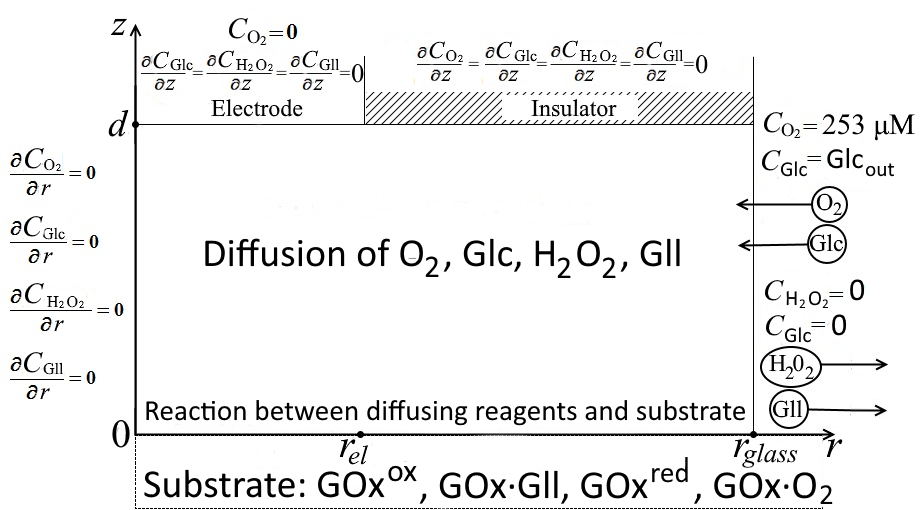
\includegraphics[width=1\linewidth]{chapter_1/Model_domain.png}
\caption{Scheme of simulation domain. All 8 reagents, boundary conditions for $C_{\text{diff}}$ and the direction of outside flux are displayed.}
\label{fig:Domain}
\end{figure}

Measurements of SECM acting in the redox-competition mode are changed into the scheme (\ref{fig:Domain}) due to the radial symmetry around the central axis of the electrode. Radial symmetry is a standard assumption in SECM modelling, though the case of off-centered UME was also investigated \cite{cornut2011accurate}.

According to the second Fick’s law \cite{laforge2008physicochemical}, diffusion processes are expressed by the system of partial differential equations (PDE):
\begin{equation}
  \begin{aligned}\label{eq:reakc_eq1}
  \frac{\partial C_{O_2}}{\partial t} &= D_{O_2}\,\Delta C_{O_2},\\
  \frac{\partial C_{Glc}}{\partial t} &= D_{Glc}\,\Delta C_{Glc},\\
  \frac{\partial C_{H_2 O_2}}{\partial t} &= D_{H_2 O_2} \,\Delta C_{H_2 O_2},\\
  \frac{\partial C_{Gll}}{\partial t} &= D_{Gll}\,\Delta C_{Gll},  \quad for\; 0<t\leq T,\; 0<z<d,\; 0<r<r_{glass},
  \end{aligned}
\end{equation}
where:
\begin{itemize}
  \item[] $C_{O_2}$, $C_{Glc}$, $C_{H_2 O_2}$ and $ C_{Gll}$ are concentrations of diffusing reagents and expressed as functions of time $t$ and spatial coordinates $z$ and $r$. Notation $C_{\text{diff}} = C_{\text{diff}} \left( t, z, r \right) = \left( C_{O_2}, C_{Glc}, \allowbreak C_{H_2 O_2}, \allowbreak C_{Gll} \right)$ was used when 4 diffusing re\-agents were considered together.
  \item[] $D_{O_2}$, $D_{Glc}$, $D_{H_2 O_2}$ and $D_{Gll}$ are diffusion coefficients of \ce{O2}, Glc, \ce{H2O2} and Gll.
  \item[] $d$ is the distance between the enzyme-modified surface and the electrode, which is varying from \SIrange{1}{120}{\um} as shown in Fig. \ref{fig:Domain}.
  \item[] $r_{glass} = \SI{80}{\um}$ is the radius of insulated area, $r_{el} = \SI{5}{\um}$ is the radius of electrode.
  \item[] $T$ is the duration of a computational experiment measured in seconds (the evaluation of this parameter is further explained in the next section).
  \item[] The Laplace operator $\Delta$ for concentration function $C$ in cylindrical coordinates with radial symmetry is
  \begin{equation*}
  \Delta C = \frac{1}{r}\frac{\partial }{\partial r} \left( r\frac{\partial C }{\partial r} \right) + \frac{\partial^{2} C}{\partial z^{2}}.
  \end{equation*}
\end{itemize}



\chapter*{General conclusions - Bendrosios išvados }
\label{cha:concl}
\addcontentsline{toc}{chapter}{\MakeUppercase{General conclusions - Bendrosios išvados}} 


...




\backmatter

\restoreParagraph
\pagestyle{plain} 
% [file: bibliography.tex, started: 22-Jun-2005]
%
% PhD Thesis - top level LaTeX source file.
%
% DESCRIPTION
%   This file includes Bibliography chapter of the PhD Thesis. 
%
% CHANGES
%   2005.06.22  *  Started.
%   2008.03.18  *  Adapted to IZ.
%   2020. ...   *  Pagal VU 2017 stand 

%\chapter{Bibliography}
%	\label{chapter:Bibliography}

\chapter*{Bibliography - Literatūros sąrašas}
\label{cha:bibliography}
\addcontentsline{toc}{chapter}{\MakeUppercase{Bibliography - Literatūros sąrašas}}
\phantomsection %The \phantomsection command is needed to create a link to a place in the document that is not a figure, equation, table, section, subsection, chapter, etc.
% \parammarks{Bibliography}
	
%\bibliographystyle{plainnat}  %Sitas buvo originaliame sablone, bet galbut patogiau su santrumpomis
% \nocite{*} %All sources from bibliography wiill be included in the disertaciotn. Removes warning Package natbib Warning: Empty `thebibliography' environment on input line

\bibliographystyle{abbrvnat} %Bibliografijoje vardai su santrumpomis
\pagestyle{plain}
\bibliography{thesis_bibliography}

%-------------- Baigiasi pagrindine disertacijos dalis  ------------------
%-------------- End of main thesis part  ------------------

\IZParagraph

%\addcontentsline{toc}{chapter}{\numberline{}Vocabulary - \v{Z}odyn\.elis}
	
\parammarks{Vocabulary - \v{Z}odyn\.elis}

\chapter*{Vocabulary - \v{Z}odyn\.elis}
\label{cha:zodynas}

\begin{compactitem}[]
\item base learner - bazinis klasifikatorius 
\item baseline - bazinis metodas 
\item change point - poky\v{c}io ta\v{s}kas 
\item concept drift - koncepcijos pokytis
\item context aware - kontekstinis 
\item data mining - duomen\k{u} gavyba 
\item data source - duomen\k{u} \v{s}altinis
\item gradual drift - palaipsnis pokytis 
%incremental drift - 
\item instance - vektorius
\item instance based learning - mokymas pagal vektorius 
\item label - klas\.e
\item moving average - slenkantis vidurkis 
\item peer methods - lyginamieji metodai 
\item recurring concepts - pasikartojantis pokytis (pasikartojan\v{c}ios koncepcijos)
\item sequential learning - mokymas paeiliui
\item source - \v{s}altinis
\item sudden drift - staigus pokytis
\item supervised learning - mokymas su mokytoju
\item training window - mokymo langas 
\item unsupervised learning - mokymasis 
\end{compactitem}


  %Jeigu reikia ideti zodyna, pasitikrinti, kur jis turi buti
\appendix  
%\renewcommand{\thesection}{\alph{section}}
	
\chapter*{Appendix / Priedai}
\label{cha:appendixA}
\addcontentsline{toc}{chapter}{\MakeUppercase{Appendix / Priedai}}
\phantomsection %The \phantomsection command is needed to create a link to a place in the document                      that is not a figure, equation, table, section, subsection, chapter, etc.

% \parammarks{Appendix}

%\index{Algorithms}

\renewcommand{\thefigure}{A.\arabic{figure}}   
\setcounter{figure}{0}
\renewcommand{\thetable}{A.\arabic{table}}
\setcounter{table}{0}
%jeigu yra dar ko nors, pvz algoritmu, teor ir pan, irgi reikia atnaujinti

\section{Algorithms}

In this Appendix we present pseudo codes and the settings used for the peer algorithms, which we implemented and used in experimental evaluation through the thesis. For consistency, the algorithms were named using the first three letters of the surname of the first author.
  %pdfe negraziai atrodo bookmarkai taip pridejus, bet pakenciama

%Change default parameters for Lithuanian language
\setcounter{section}{0}   %šita automatiškai atnaujina \appendix komanda
\renewcommand*{\thesection}{S.\arabic{section}}
\renewcommand{\thechapter}{S}
\renewcommand{\thefigure}{S.\arabic{figure}}   %raidė S įhardcodinta. Galima švelniau pvz su komanda \thechapter
\setcounter{figure}{0}
\renewcommand{\theequation}{S.\arabic{equation}}
\setcounter{equation}{0}
\renewcommand{\thetable}{S.\arabic{table}}
\setcounter{table}{0}
%jeigu yra dar ko nors, pvz algoritmu, teor ir pan, irgi reikia atnaujinti

\lithuanian   %nustatome lietuviu kalba
\sisetup{output-decimal-marker = {,}}  %lietuviski kableliai ir pan
\sisetup{exponent-product=\ensuremath{\cdot}}


\phantomsection
\chapter*{Summary in Lithuanian / Summary in English}
\label{cha:summary_lt}
\addcontentsline{toc}{chapter}{\MakeUppercase{Summary in Lithuanian - Summary in English}}

% NOTES to the author
% For chapter naming, please use APA style https://titlecapitalize.com/title-case-styles/
    % APA, or American Psychological Style, is one of the most commonly used title case styles in academia. It’s mainly used for research papers in social and behavioral sciences. 
    
    % Its title case rules are also easy enough to remember and follow. Capitalize all major words (nouns, pronouns, verbs, adjectives) in your title, as well as prepositions and conjunction with four or more letters. If your title includes a hyphenated word, capitalize both the initial letters before and after the hyphen. Lastly, the first word after a colon or dash is also capitalized when you’re following the APA style of capitalization for your title or headings.

\chapter*{Introduction / Įvadas}
\label{cha:intro_lt}
\addcontentsline{toc}{chapter}{\MakeUppercase{Introduction / Įvadas}} 

The dissertation must be an original scientific work that substantiates the research problem, defines the \textbf{relevance and purpose of the research work, formulates the goal and objectives of the thesis, indicates the novelty of the scientific work, presents defending statements of the thesis}, reviews the research conducted on the topic of the dissertation in the world (abroad and in Lithuania) and their results, presents the applied research methodology (methods), research results discussed, their reliability and relationship with the data of other researchers, conclusions formulated and other important aspects, in the dissertation's opinion.


\textbf{In Lithuanian}. Disertacija turi būti originalus mokslinis darbas, kuriame pagrindžiama \textbf{tiriamoji problema, apibrėžtas darbo aktualumas, tikslas, suformuluoti sprendžiami uždaviniai, nurodytas mokslinio darbo naujumas, ginami disertacijos teiginiai}, apžvelgti disertacijos tema pasaulyje (užsienyje ir Lietuvoje) atlikti tyrimai ir jų rezultatai, pristatyti taikyta tyrimų metodika (metodai), aptarti tyrimų rezultatai, pagrįstas jų patikimumas ir santykis su kitų tyrėjų duomenimis, suformuluotos išvados ir kiti, disertanto nuomone, svarbūs aspektai.


\phantomsection % Removes warning from hyperref package
\section*{Research Area / Tyrimų sritis}
\addcontentsline{toc}{section}{Research Area / Tyrimų sritis} 

In this section, we recommend briefly introducing the readers to the field of research, which is directly related to the research problem and the aim of the dissertation. Present the current situation in this research area, name the important and relevant research conducted in this area, and present their results. You can attach the research problem section to this section.

\textbf{In Lithuanian}.
Šiame skyrelyje rekomenduojame trumpai skaitytojus supažindinti su tyrimų sritimi, kuri tiesiogiai siejasi su su disertacijos problema ir tikslu. Pristatykite kokia yra dabar situacija šioje srityje, įvardinkite svarbius ir aktualius šioje srityje vykdomus tyrimus ir prisatykite jų rezultatus. Prie šio skyrelio galite prijunti tyrimo problemos skyrelį.

\section*{Research Problem / Tyrimo problema}
\addcontentsline{toc}{section}{Research Problem / Tyrimo problema} 

Definition. A perceived gap between the existing state and a desired state, or a deviation from a norm, standard, or status quo (Bussiness Dictionary\footnote{https://www.bussinessdictionary.com/definition/problem}).

Also:
\begin{itemize}
    \item A problem is a statement, in mathematics or physics, that indicates the need to do something.
    \item The problem is a complex unsolved question. 
    \item A scientific problem can be solved using the steps of the scientific method (e.g. experiments).
\end{itemize}
Before formulating a scientific problem, it is recommended to define the research object and formulate the problem using its concepts.


\textbf{In Lithuanian}. Apibrėžimas. \textbf{Problema} – tai tarpas tarp esamos būsenos ir siekiamos būsenos, arba nukrypimas nuo normos, standarto ar status quo.
Taip pat:
\begin{itemize}
    \item Problema – teiginys, matematikoje ar fizikoje, nurodantis poreikį kažką padaryti.
    \item Problema – sudėtingas neišspręstas klausimas. 
    \item Mokslinė problema – tai klausimas, kuris gali būti atsakytas naudojant mokslinius metodus (pvz., atliekant eksperimentus).
\end{itemize}
Prieš formuojant mokslinę promblemą rekomenduojama apsibrėžti tyrimo objektą ir naudojantis jo sąvokomis suformuluoti problemą.


\section*{Actuality / Darbo aktualumas}
\addcontentsline{toc}{section}{Actuality / Darbo aktualumas} 

The actuality of the research topic is the degree of its importance at the given moment and in this situation for solving these problems, a question or a problem\footnote{\url{https://en.ppt-online.org/424459}}.

In order to show the actuality of the research, you need:
\begin{itemize}
    \item to formulate the research problem
    \item to indicate contradictions found in science or practice that define the research problem
    \item to describe the current situation of the problem with a solution to the problem (is anyone still solving it?)
    \item to describe the importance of research work to society
    \item to generalize and to summarize the best results.
\end{itemize}

\textbf{In Lithuanian}.
Tyrimo temos aktualumas yra sprendžiamos problemos ar klausymo svarbos laipsnis šiuo momentu ir šiuoje situacijoje sprendžiant tyrimo sirties problemas.
Kad parodyti darbo aktualumą reikia:
\begin{itemize}
    \item suformuluoti tyrimo problemą,
    \item nurodyti prieštaravimus kurie aptinkami moksle arba praktikoje, kurie apibrėžia tyrimo problemą, 
    \item apibūdinti esamą problemos situaciją su problemos sprendimu (ar ją kas nors vis dar sprendžia?),
    \item darbo reikšmingumą visuomenei,
    \item apibendrinti geriausius rezultatus.
\end{itemize}


\section*{Research Object / Tyrimo objektas}
\addcontentsline{toc}{section}{Research Object / Tyrimo objektas} 

\textbf{Research object} or research subject is a thing (e.g. algorithm, person, data type) that is used in your research. The research object connects different research contexts: data, analysis tools, hypotheses, experiments, defending statements, and general conclusions. We recommend identifying from 3 to 5 main research concepts and formulating a coherent sentence from them as a research object.
These concepts should also be used in the thesis title and objective. You can read more about how to identify the object of your research on  \url{http://edutechwiki.unige.ch/en/Methodology_tutorial_-_finding_a_research_subject}.

\textbf{In Lithuanian}. \textbf{Tyrimo objektas} (angl. research object, research subject) – daiktas (pvz. algoritmas, asmuo, duomenų tipas), kuris naudojamas detaliame tyrime. Tyrimo objektas susieja skirtingus tyrimo kontekstus: duomenis, analizės įrankius, hipotezes, eksperimentus, ginamuosius teiginius ir išvadas. Rekomenduojame identifikuoti nuo 3 iki 5 pagrindinių tyrimo konceptų ir iš jų suformuluoti nuoseklų sakinį.
Šie konceptai taip pat turėtų būti panaudoti disertacijos pavadinime ir tiksle. Daugiau apie taip kaip identifikuoti savo tyrimo objektą galima paskaityti \url{http://edutechwiki.unige.ch/en/Methodology_tutorial_-_finding_a_research_subject}.



\section*{Research Aim and Objectives / Tyrimo tikslas ir uždaviniai}
\addcontentsline{toc}{section}{Research Aim and Objectives / Tyrimo tikslas ir uždaviniai} 

The goal of science is an action that is performed to solve a defined scientific problem of your research.
The following types of scientific goals are distinguished\footnote{\url{https://opentext.wsu.edu/carriecuttler/chapter/goals-of-science/}}:
\begin{itemize}
    \item The first and most basic goal of science is \textbf{to describe}.
    \item The second goal of science is \textbf{to predict}.
    \item The third and ultimate goal of science is \textbf{to explain}.
\end{itemize}
When defining the main goal of the dissertation, it is recommended to think about what you managed \textbf{to create} in your dissertation. Thus, defining the goal will make it easier for you to describe the novelty and originality of the research work. 
If your research aims to create a solution, a tool, or an algorithm, it will also be related to scientific aims: to describe, predict, or explain.

For the aim of research, the only requirement is \textbf{it must be measurable}.

Research objectives are smaller actions required to achieve the aim. They must also be measurable. 
The research objective must be relevant, related to the aim, feasible, logical, measurable, and unambiguous.
When executing the objective, we aim to find answers to questions or test research hypotheses.

It is recommended that each objective relates to at least one defending statement and at least one thesis general conclusion. This way you will achieve consistency and integrity of your work. It is recommended that the number of research tasks should be between 3 and 5.

\textbf{In Lithuanian}. 
Mokslo tikslas tai veiksmas kuris atliekamas norint išspręsti apibrėžtą savo tyrimo mokslinę problemą. 
Yra išskiriami šie mokslo tikslų tipai:
\begin{itemize}
    \item Pirmas ir bazinis mokslo tikslas – „\textbf{Aprašyti}/apibūdinti/apibrėžti“ (angl. to describe).
    \item Antras mokslo tikslas – „\textbf{Prognozuoti}“ (angl. to predict“).
    \item Trečiasis ir pagrindinis mokslo tikslas „\textbf{Paaiškinti}/Suprasti“ (angl. to explain/understand).
\end{itemize}

Konstruojant pagrindinį disertacijos tiklsą rekomenduojama pagalvoti, o ką jūsų darbe pavyko  \textbf{sukurti}, taip apibrėžiant tikslą jums lengviau bus aprašyti darbo naujumą ir orgiginalumą. Darbo tikslas, kaip sukurtas sprendimas, įrankis ar algoritmas siesis ir mokslo tikslais: aprašyti, prognozuoti ar paaiškinti.

Tyrimo tikslui, keliamas vienintelis reikalavimas - \textbf{jis turi būti pamatuojamas}.

Tyrimo uždaviniai tai mažesni veiksmai reikalingi užsibrėžtam tikslui pasiekti. Jie taip pat turi būti  pamatuojami. 
Mokslinis uždavinys turi būti, aktualus, susijęs su tikslu, įvykdomas, logiškas, pamatuojamas, nedviprasmiškas.
Spręsdami uždaviniais mes siekiame surasti atsakymus į klausimus arba patikrinti tyrimo hipotezes.

Rekomenduojama, kad kiekvienas uždavinys sietųsi su bent vienu ginamuoju teiginiu ir su bent su viena disertacijos išvada. Taip pasieksite darbo nuoseklumo ir vientisumo. Rekomenduojama, kad tyrimo uždavinių kiekis būtų nuo  3 iki 5.

\section*{Research Methods / Tyrimo metodai}
\addcontentsline{toc}{section}{Research Methods / Tyrimo metodai} 

Research methods are specific procedures for collecting and analyzing data. Developing your research methods is an integral part of your research design. For more about available research methods, please read on \url{https://www.scribbr.com/category/methodology/}.

\textbf{In Lithuanian}. 
Tyrimo metodai – tai specifinės duomenų rinkimo ir analizės procedūros. Tyrimo metodų kūrimas yra neatsiejama jūsų tyrimo plano dalis. Daugiau tyrimo metodus, skaitykite \url{https://www.scribbr.com/category/methodology/}.


\section*{Scientific Novelty / Mokslinis darbo naujumas} %Scientific Contribution of the Research
\addcontentsline{toc}{section}{Scientific Novelty / Mokslinis naujumas} 

This is one of the main requirements for the dissertation. This means that the dissertation must have a solution to a new scientific problem or a new development that allows expanding the existing boundaries of knowledge in a certain branch of science.

A job is new if:
\begin{itemize}
 \item it is a new interesting question (problem) or topic,
 \item it is a little researched question (problem) or not studied in depth.
\end{itemize}

Novelty can be associated with the reuse of old ideas in new conditions, new fields of science, or practice.

The novelty of the work can be achieved by the following methods:
\begin{itemize}
 \item Introduction of new previously unused sources (methods, laws, theorems) into the existing field of science and their subsequent analysis.
 \item New interpretation of existing and known sources and addition or correction of existing knowledge.
 \item Researching little-understood or analyzed sources of old information and their aspects.
\end{itemize}


\textbf{In Lithuanian}. Tai vienas iš pagrindinių reikalavimui disertacijos temai. Tai reiškia kad darbas turi turėti sprendimą naujai mokslinei problemai, arba nauja plėtra kuri leidžia praplėsti egzistuojančias tam tikros mokslo šakos žinių ribas.
Darbas yra naujas, jeigu:
\begin{itemize}
    \item tai naujas įdomus klausimas (problema) ar tema,
    \item tai mažai tyrinėtas klausimas (problema) ar netyrinėtas giliai.
\end{itemize}

Naujumas gali būti susietas su senų idėjų pakartotiniame panaudojimu naujose sąlygose, naujose mokslo ar praktikos srityse.

Darbo naujumas gali būti pasiektas šiais metodais:
\begin{itemize}
    \item Naujų ankščiau nenaudotų šaltinių (metodai, dėsniai, teoremos) įvedimas į esamą mokslo sritį ir vėlesnė jų analizė.
    \item Nauja esamų ir žinomų šaltinių interpretacija ir esamų žinių papildymas ar pataisymas.
    \item Tyrinėjimas mažai suvoktus ar išanalizuotus senos informacijos šaltinius, jų aspektus.
\end{itemize}



\section*{Practical Significance / Praktinė darbo vertė}  %Gali būti impact, kuris žodis geresnis? ar Practical Value of the Research
\addcontentsline{toc}{section}{Practical Significance / Praktinė darbo vertė} 

In this section, discuss the practical benefits of the results of this dissertation work. Describe where and how they were, are, or can be applied in practice. Or indicate how they contribute to solving practical problems.

\textbf{In Lithuanian}. 
Šiame skyrelyje pakalbėkite apie šio disertacijos darbo rezultatų praktinę naudą. Aprašykite kur ir kaip jie buvo, yra ar gali būti pritaikyti praktikoje. Arba nurodykite kaip jie prisideda prie praktinių problemų sprendimo.

\section*{Statements to be Defended / Ginamieji teiginiai}
\addcontentsline{toc}{section}{Statements to be Defended / Ginamieji teiginiai}

According to the recommendations set by the Lithuanian Science Council for the structure of the dissertation, the introduction must contain defending statements, which must also be reflected in the conclusions.
There are no more detailed requirements defining what the defending statements are or how many of them there should be - so it is enough to remind you of the previously mentioned advice to read theses defended in a specific discipline and participate in their defenses.

The answer to the question of what are defending statements can be found in another way - by clarifying the concept of "defending statement".
\begin{itemize}
    \item First, it must be a statement (not a question).
    \item Second, it must be a statement that is defended in the thesis, i.e. a statement that is not self-evident and requires justification. 
\end{itemize}
A defending statement is just the equivalent of a thesis with a different name - it states what and how it is intended to be proved.
In many cases, the equivalent of a defending statement can be a hypothesis - in the dissertation, we test assumptions about an expected relationship.

The recommended number of defending statements is from 3 to 5. They must also be related to the research objectives and conclusions.

\textbf{In Lithuanian}. 
Pagal  Lietuvos  mokslo  tarybos  nustatytas  rekomendacijas  disertacijos struktūrai, įvade turi būti suformuluoti ginamieji teiginiai, kurie taip pat jie turi atsispindėti išvadose. 
Detalesnių reikalavimų, apibrėžiančių, kas  yra  ginamieji  teiginiai  ar kiek jų  turėtų būti,  nėra nustatyta – todėl telieka priminti jau anksčiau minėtą patarimą skaityti konkrečioje disciplinoje gintas disertacijas ir dalyvauti jų gynimuose (Doktorantūros studijų kokybės valdymas, metodinė medžiaga doktorantų vadovams ir doktorantams, VU, 2013 m.\footnote{\url{https://www.mii.vu.lt/files/doc/lt/doktorantura/dokumentu_sablonai/doktoranturos_studiju_kokybes_valdymas_metodine_medziaga_doktorantu_vadovams_ir_doktorantams1.pdf}
}).

Atsakymo į klausimą, kas yra ginamieji teiginiai, galima ieškoti ir kitu keliu – išsiaiškinant „ginamojo teiginio“ sąvoką. 
\begin{itemize}
    \item Pirma, tai turi būti teiginys (o ne klausimas). 
    \item Antra, tai turi būti teiginys, kuris disertacijoje yra ginamas, t.y. teiginys, kuris nėra savaime akivaizdus ir kurį reikia pagrįsti. 
\end{itemize}
Ginamasis teiginys yra tik kitaip įvardintas tezės ekvivalentas – juo įvardijama, kas ir kaip ketinama įrodinėti. 
Ginamojo teiginio ekvivalentu daugeliu atveju gali būti hipotezės – disertacijoje tikrinami spėjimai apie numatomą priežastinį ryšį.

Rekomenduojamas ginamųjų teiginių kiekis nuo  3 iki 5. Ir jie turi sietis su turimo uždaviniais ir darbo išvadomis.


\section*{Approbation and Publications of the Research/ Tyrimo aprobavimas ir publikavimas} %Darbo rezultatų aprobavimas
\addcontentsline{toc}{section}{Approbation and Publications of the Research/ Tyrimo aprobavimas ir publikavimas} 

Your dissertation must meet the formal requirements, i.e., the results presented in the dissertation had to be published in at least two journals indexed in the Web Of Science database and discussed at two international conferences.
In this section, a list of publications published in the Web Of Science database (same as \nameref{cha:publications}) and list of all other publication should be presented. Additionally, provide a list of all scientific events where you have given presentations on the topic of the dissertation.

\textbf{In Lithuanian}. 
Jūsų disertacija turi tenkinti formalius reikalavimus, t.y. disertacijoje pristatomi rezultatai turėjo būti išspausdinti bent dviejuose žurnaluose indeksuojamuose Web Of Science duomenų bazėje, ir aptarti bend dvejose tarptautinėse konferencijose.
Šiame skyrelyje pateiktite sąrašą visų disetacijos tema išspaudintų darbų iš jų išskiriant publikacijas pakslebtas Web Of Science duomenų bazėje (tas pats kaip ir skyriuje \nameref{cha:publications}). Papidlomai pateikite sąrašą visų mokslinių renginių kuriuose skaitėte pranešimus disertacijos tema.


\section*{Outline of the Thesis/ Disertacijos strukūra}
\addcontentsline{toc}{section}{Outline of the Thesis/ Disertacijos strukūra} 

In this section, present the main sections of the thesis and the overall size of the thesis.

This doctoral thesis consists of an introduction, ... chapters, conclusions, and a summary in the Lithuanian language. The introduction section provides an introduction to the research and an overview of the dissertation. The first chapter is ...

... bibliographic references are included at the end of the thesis. The disertation consist of ... pages, ... figures and ... tables.


\textbf{In Lithuanian}. 

Šiame skyrelyje pristatykite pagdindinius disertacijos skyrius ir bendrą disertacijos apimtį.



\textbf{Note} Please translate all parts of the introduction to Lithuanian and put them into the \verb|chapter_intro_lt.tex| file.
\textbf{In Lithuanian}. \textbf{Pastaba}Angliško ir lietuviško įvado turinys turi būti identiškas turinio prasme. Išverstą tekstą patalpinkite \verb|chapter_intro_lt.tex| failą.

% !TEX encoding = UTF-8 Unicode

\pagestyle{plain}

%\lithuanian

\phantomsection % Removes warning form hyperref package
\section*{Tyrimų sritis}
\addcontentsline{toc}{section}{Research Area / Tyrimų sritis}

Pasitelkus kompiuterinį modeliavimą disertacijoje tiriamos su\-dė\-tin\-gos cheminės ir biofizikinės sistemos, kurios yra aprašomos dalinių išvestinių lygtimis (DIL) su netiesinėmis kraštinėmis sąlygomis ir DIL sudėtingos geometrijos (nestačiakampėse) srityse. Šios DIL sprendžiamos baigtinių skirtumų metodu ir kitais skaitiniais algoritmais. 

%Disertacijoje tiriamos sudėtingos cheminės ir biofizikinės sistemos naudojant kompiuterinį modeliavimą. Šios sistemos yra aprašomos dalinių išvestinių lygtimis (DIL) su netiesinėmis kraštinėmis sąlygomis ir DIL sudėtingos geometrijos (nestačiakampėse) srityse. Šios DIL sprendžiamos baigtinių skirtumų metodu ir kitais skaitiniais algoritmais.  
%The study is focused on computer modelling of complex chemical and biophysical systems, which are described by partial differential equations (PDEs) with nonlinear boundary conditions and PDEs in various complex (non-rectangular) domains. Differential problems are solved using numerical methods
%Tyrimas skirtas išspręsti dalinių išvestinių lygtims (DIL) su netiesinėmis kraštinėmis sąlygomis sistemas ir išspręsti DIL sudėtingos geometrijos (nestačiakampėse) srityse, naudojant skaitinius metodus.

DIL sprendimo su netiesinėmis kraštinėmis sąlygomis problemos kyla dėl cheminių ir biologinių procesų matematinio modeliavimo. 
Tyrimai nestačiakampėse srityse yra aktualūs dėl poreikio įvertinti matavimo prietaisų paklaidas, atsirandančias dėl geometrijos nukrypimo nuo standarto.
%Tyrimai nestačiakampėse srityse yra aktualūs dėl poreikio modeliuoti nukrypimus nuo normos įrangoje, naudojamoje cheminiams ir biologiniams eksperimentams. 
DIL netiesinės sistemos yra pritaikytos tyrinėti chemoterapinių vaistų patekimą į audinius.





\section*{Tikslas}
\addcontentsline{toc}{section}{Tikslas} 
...





%--------------- SECM Redox reakciju skyrius ---------------------------------
%--------------------------------------------------------------------------

\section{SECM modeliavimas oksidacijos-redukcijos konkurencijos režime}
\label{sec:santr_reakc}



\subsection{Matematinis modelis}

Dėl simetrijos aplink centrinę elektrodo ašį modelis užrašomas cilindrinėse koordinatėse. Cilindro formos srityje atliekami SECM matavimai yra pakeisti į 2D sritį \ref{fig:santr_Domain} pav.


\begin{figure}[ht!]
\centering
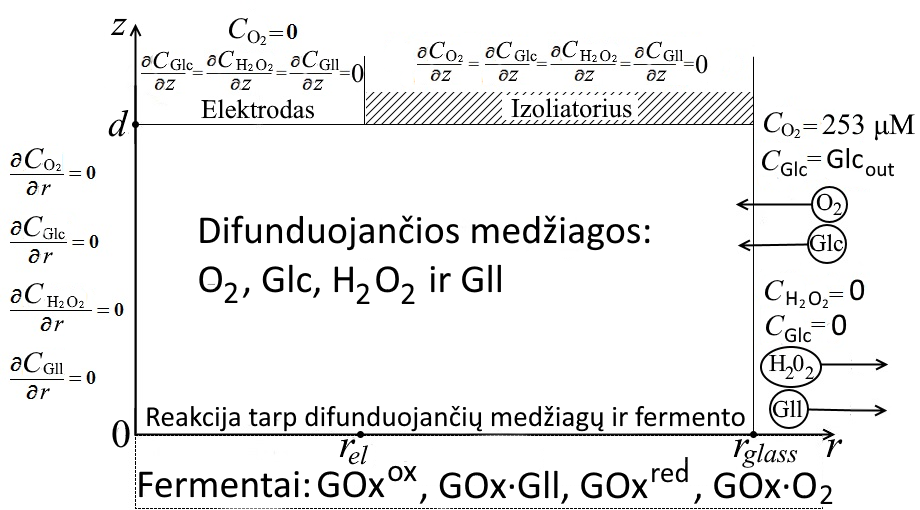
\includegraphics[width=0.8\linewidth]{summary/Model_domainLT.png}
\caption{Modeliavimo srities schema. Pavaizduotos $8$ modeliuotos medžiagos - $4$ difunduojantys reagentai bei $4$ fermento GOx formos, kraštinės sąlygos 4-ioms difunduojančioms medžiagoms ir išorinis srautas.}
\label{fig:santr_Domain}
\end{figure}

Difuzijos procesai išreiškiami antruoju Fiko dėsniu:
\begin{equation}
  \begin{aligned}\label{eq:santr_eq1}
  \frac{\partial C_{O_2}}{\partial t} &= D_{O_2}\,\Delta C_{O_2},\\
  \frac{\partial C_{Glc}}{\partial t} &= D_{Glc}\,\Delta C_{Glc},\\
  \frac{\partial C_{H_2 O_2}}{\partial t} &= D_{H_2 O_2} \,\Delta C_{H_2 O_2},\\
  \frac{\partial C_{Gll}}{\partial t} &= D_{Gll}\,\Delta C_{Gll},  \quad 0<t\leq T,\; 0<z<d,\; 0<r<r_{glass}.
  \end{aligned}
\end{equation}
Šiose lygtyse:
\begin{itemize}
  \item[] $C_{O_2}$, $C_{Glc}$, $C_{H_2 O_2}$ ir $C_{Gll}$ yra atitinkamų difunduojančių re\-a\-gen\-tų koncentracijos, kurios išreiškiamos kaip laiko $t$, er\-dvi\-nių ko\-or\-di\-na\-čių $z$ ir $r$ funkcijos. 
  \item[] $D_{O_2}$, $D_{Glc}$, $D_{H_2 O_2}$ ir $D_{Gll}$ yra difuzijos koeficientai.
  \item[] $d$ yra atstumas tarp fermentu modifikuoto paviršiaus ir elektrodo. Skaitinio eksperimento metu $d$ keičiamas nuo $\SI{1}{\um}$ iki $\SI{120}{\um}$. Tai atitinka elektrodo stumdymą aukštyn ir žemyn cheminio eksperimento metu.
  \item[] $r_{glass} = \SI{80}{\um}$ yra izoliuotos srities spindulys.
  \item[] $T$ yra skaičiavimo eksperimento trukmė, matuojama sekundėmis.
  \item[] Laplaso operatorius $\Delta$ cilindrinėse koordinatėse su centrine simetrija yra
  \begin{equation*}
  \Delta C = \frac{1}{r}\frac{\partial C }{\partial r} \left( r\frac{\partial C }{\partial r} \right) + \frac{\partial^{2} C}{\partial z^{2}}.
  \end{equation*}
\end{itemize}


\chapter*{General conclusions / Bendrosios išvados }
\label{cha:concl_lt}
\addcontentsline{toc}{chapter}{\MakeUppercase{General conclusions / Bendrosios išvados}} 

It is recommended that these conclusions relate directly to the objectives and defending statements of the thesis. 
The conclusions should accurately reflect the results obtained in the dissertation work.
The recommended number of conclusions is 3-5.

\textbf{Note}. Please do a direct translation of the conclusion to Lithuanian language and put them to the \verb|chapter_concl_lt.tex|.


\textbf{In Lithuanian} Šiame skyriuje pateikite sąrašą pagrindinių disertacijos išvadų. Rekomenduojama, kad šios išvados tiesiogiai sietųsi su darbo uždaviniais ir ginamaisiais teiginiais. Išvadose turėtų tiksliai atsispindėti rezultatai gauti disertacijos darbe. 
Rekomenduojamas išvadų kiekis 3-5.

\textbf{Pataba}.Jeigu disertaciją rašote lietuviškai, tuomet išvadas išverskite į anglų kalbą ir pateikite \verb|chapter_concl.tex| faile, kuris būtų naudojamas angliškoje disertacijos santraukoje.
Jeigu disertaciją rašote angliškai, tuomet išverskite į lietuvių kalbą ir pateikite \verb|chapter_concl_lt.tex| faile.

\british  %griztame prie anglu kalbos
%%%%%%%%%%%%%%%%%%%%%%%%%%%%%%%%%%%%%%%%%%%%%%%%%%%%%%%%%%%%%%%%%%%%%%%%%%%%%%%%%%%%%%%%%%%%%%
%% CV is not required in the dissertation body, but it is required in the dissertation summary
%% CV neprašo įdėti į disertacijos turinį, bet prašo įdeti po santraukos
\chapter*{Curriculum Vitae - Gyvenimo aprašymas}
\label{cha:cv}
\addcontentsline{toc}{chapter}{\MakeUppercase{Curriculum Vitae - Gyvenimo aprašymas}}
% \parammarks{Curriculum Vitae}


Vardas Pavardė graduated from ... 

The author's curriculum vitae should be at max one paragraph long.    %Nors cv reikalavimo nera, VU doktoranturos skyrius turetu paprasyti prideti po santraukos gyvenimo aprasyma

\backmatter
\IZParagraph 
%%%%%%%%%%%%%%%%%%%%%%%%%%%%%%%%%%%%%%%%%%%%%%%%%%%%%%%%%%%%%%%%%%%%%%%%%%%%%%%%%%%%%%%%%%%%%%
%% Acknowledgements / Padėka

\chapter*{Acknowledgements - Padėka}
\label{cha:acknowledgements}
\addcontentsline{toc}{chapter}{\normalfont\MakeUppercase{Acknowledgements - Padėka}}

\phantomsection %The \phantomsection command is needed to create a link to a place in the document that is not a figure, equation, table, section, subsection, chapter, etc.

%%%%%%%%%%%%%%%%%%%%%%%%%%%%%%%%%%%%%%%%%%%%%%%%%%%%%%%%%%%%%%%%%%%%%%%%%%%%%%%%%%%%%%%%%%%%%%
%%  Texts of the acknowledgements / Padėkos tekstas

Your acknowledgment text goes here. Try to keep it within one page.

It is not required / Padėka neprivaloma.

% Use as it is necessary
% {\flushright  
%     \thesisAuthorName \ \thesisAuthorSurname \\ Vilnius\\ \today\\ 
% }  %Neprivalomas

\chapter*{List of publications - Publikacijų sąrašas}
\label{cha:publications} 
\addcontentsline{toc}{chapter}{\MakeUppercase{List of publications - Publikacijų sąrašas}}	
%\parammarks{\chapter*{List of publications - Publikacijų sąrašas}}

%Čia galima įdėti ir visą publikacijų sąrašą, jei norite
%\input{publications/author's_publications.bib}

%\index{publications} 

%Bibliografinio aprašo elementų tvarka
%Straipsnis: 
%1. pirminė atsakomybė (autoriaus vardas ir pavardė) (privaloma); 2. straipsnio antraštė ir paantraštė (privaloma); 3. žurnalo pavadinimas (privaloma); 4. žurnalo numeracija (tomas, numeris, metai) (privaloma); 5. paginacija, puslapių intervalas; 6. elektroninio straipsnio identifikatoriai arba interneto nuoroda: a) DOI numeris; b) interneto nuoroda (jeigu nėra DOI numerio).
%Knyga: 
%1. pirminė atsakomybė (autoriaus(ių) pavardė ir vardas; kolektyvo/organizacijos pavadinimas, jei tai kolektyvinis autorius) (privaloma); 2. knygos antraštė ir paantraštė (privaloma); 3. antrinė atsakomybė (vertėjai, redaktoriai, sudarytojai) (jeigu nurodyti antraštiniame lape); 4. leidimas (jeigu ne pirmas leidimas); 5. tomas (jeigu cituojamas daugiatomis leidinys); 6. serijos pavadinimas (neprivaloma); 7. skelbimo informacija (leidimo vieta, leidykla, metai) (privaloma); 8. elektroninės knygos identifikatoriai arba interneto nuoroda: a) DOI numeris; b) interneto nuoroda (jeigu nėra doi numerio).

\makeatletter
\newcommand{\authorpaperlabel}[2]{%
    \@bsphack
    \begingroup
        \def\label@name{#1}%
        \label@hook
        \protected@write\@auxout{}{
            \string\newlabel{#1}{%
                {#2} %current label
                {\thepage} %
                {\@currentlabelname}%
                {\@currentHref}%
                {}%
            } %
        }%
    \endgroup
    \@esphack
}%
\makeatother
  
\newcounter{itemnumber}
\newenvironment{publicationlist}[1]{% Prefix
\setcounter{itemnumber}{0}%
\begin{list}{\textbf{#1}}{}%
}{\end{list}}

\newcommand{\publicationentry}[2]{% Number, Text
\stepcounter{itemnumber}%
\item {[}#1.\theitemnumber{]}\ #2 \authorpaperlabel{mypaper:#1.\theitemnumber} {[#1.\theitemnumber]}%
\label{[#1.\theitemnumber]}%
}

\textbf{Articles/Straipsniai:}

\begin{publicationlist}{}
    \publicationentry{A}{Vardas, P. \& Kitas, A. Title of the book - knygos pavadinimas. (CRC Press,2024)}
    \publicationentry{A}{lorem ipsum dwa}
    \publicationentry{A}{lorem ipsum tri}
\end{publicationlist}

\textbf{Books/Knygos:}
\begin{publicationlist}{}
    \publicationentry{B}{ardas, P. \& Kitas, A. Title of the paper - straipsnio pavadinimas. {\em Biochimica Et Biophysica Acta (BBA)-Biomembranes}. \textbf{1061}, 33-38 (2024), https://www.mii.lt}
    \publicationentry{B}{lorem ipsum dwa}
    \publicationentry{B}{lorem ipsum tri}
\end{publicationlist}

\ref{mypaper:A.1}
\ref{mypaper:A.3}
\ref{mypaper:B.2}   %Publikaciju sarasas ir ju kopijos

%\restoreParagraph
%% [file: index.tex, started: 25-Aug-2005]
%
% PhD Thesis - top level LaTeX source file.
%
% DESCRIPTION
%   This file includes Index chapter of the PhD Thesis. 
%   USe command \index{keyword} to add "keyword" to the index
%
% CHANGES
%   2005.08.25  *  Started.
%   2008.03.18  *  Adapted to IZ.
%   2024.08.30  *  Fixed to fit VU dissertation template
% \chapter{Index}
% \label{chapter:Index}

\addtocontents{toc}{\protect\enlargethispage{2\baselineskip}}
\phantomsection
% \addcontentsline{toc}{chapter}{\numberline{}Index} % \numberline{} atitraukia į šalį
\addcontentsline{toc}{chapter}{\MakeUppercase{Index}}

%To add something to index please use command \index{keyword}
%Show index items in two-column style sorted by name
{\raggedright
    \printindex
}
  %indexas - nuorodos i puslapius, kur panaudota kokia svarbi savoka. Nereikalinga	

\pagestyle{empty}

\iffalse   
\begin{center}   %Jeigu truktu puslapiu. Leidykla prasys kad dalintusi is 4
NOTES
\end{center}
\newpage
\fi

\cleardoublepage



\vspace{165mm}

\begin{flushleft}
Rokas Astrauskas
	
Computer Modelling of Reaction-Diffusion Processes\\ 
in Scanning Electrochemical Microscopy and in Cell Spheroids

Doctoral Dissertation\\
Natural Sciences\\
Informatics (N 009)\\
Thesis Editor: ...


\vspace{3cm}

Reakcijos-difuzijos procesų kompiuterinis modeliavimas\\
skenuojančioje mikroskopijoje ir ląstelių sferoiduose

Daktaro disertacija\\
Gamtos mokslai\\
Informatika (N 009)\\
Santraukos redaktorė: ...


\end{flushleft}




\vspace{165mm}

{
	\vspace*{\fill}
	
	\centering
Vilnius University Press\\
9 Saulėtekio Ave., Building III, LT-10222 Vilnius\\
Email: info@leidykla.vu.lt, www.leidykla.vu.lt\\
Print run of ... copies\\
}
  %pacioje pabaigoje - darsyk pavadinimas ir leidykla

\end{document}